\section{Simulation Analysis}
\label{sec:simulation}

\subsection{Operating Point Analysis}

\subsubsection{First task}

Table~\ref{tab:op1} shows ---------------------------------

\begin{table}[H]
  \centering
  \begin{tabular}{|l|r|}
    \hline    
    {\bf Name} & {\bf Value [A or V]} \\ \hline
    \input{../sim/op1_tab}
  \end{tabular}
  \caption{Operating point. Variables v(i) are of type {\it voltage} and expressed in
    Volt; other variables are of type {\it current} and expressed in Ampere}
  \label{tab:op1}
\end{table}

The results are the same as the ones obtained using Octave. The subject will be further developed in Section~\ref{sec:conclusion}.

-----------------------------------------------
-----------------------------------------------
-----------------------------------------------
-----------------------------------------------
-----------------------------------------------
-----------------------------------------------
-----------------------------------------------
-----------------------------------------------

\subsubsection{Second task}

Table~\ref{tab:op2} ----------------------------------- 

\begin{table}[H]
  \centering
  \begin{tabular}{|l|r|}
    \hline    
    {\bf Name} & {\bf Value [A or V]} \\ \hline
    \input{../sim/op2_tab}
  \end{tabular}
  \caption{Operating point. Variables v(i) are of type {\it voltage} and expressed in
    Volt; other variables are of type {\it current} and expressed in Ampere}
  \label{tab:op2}
\end{table}

-----------------------------------------------
-----------------------------------------------
-----------------------------------------------
-----------------------------------------------
-----------------------------------------------
-----------------------------------------------
-----------------------------------------------
-----------------------------------------------



\subsubsection{Third task}

Figure~\ref{fig:trans_al3} ----------------------------------- 

\begin{figure}[H] \centering
  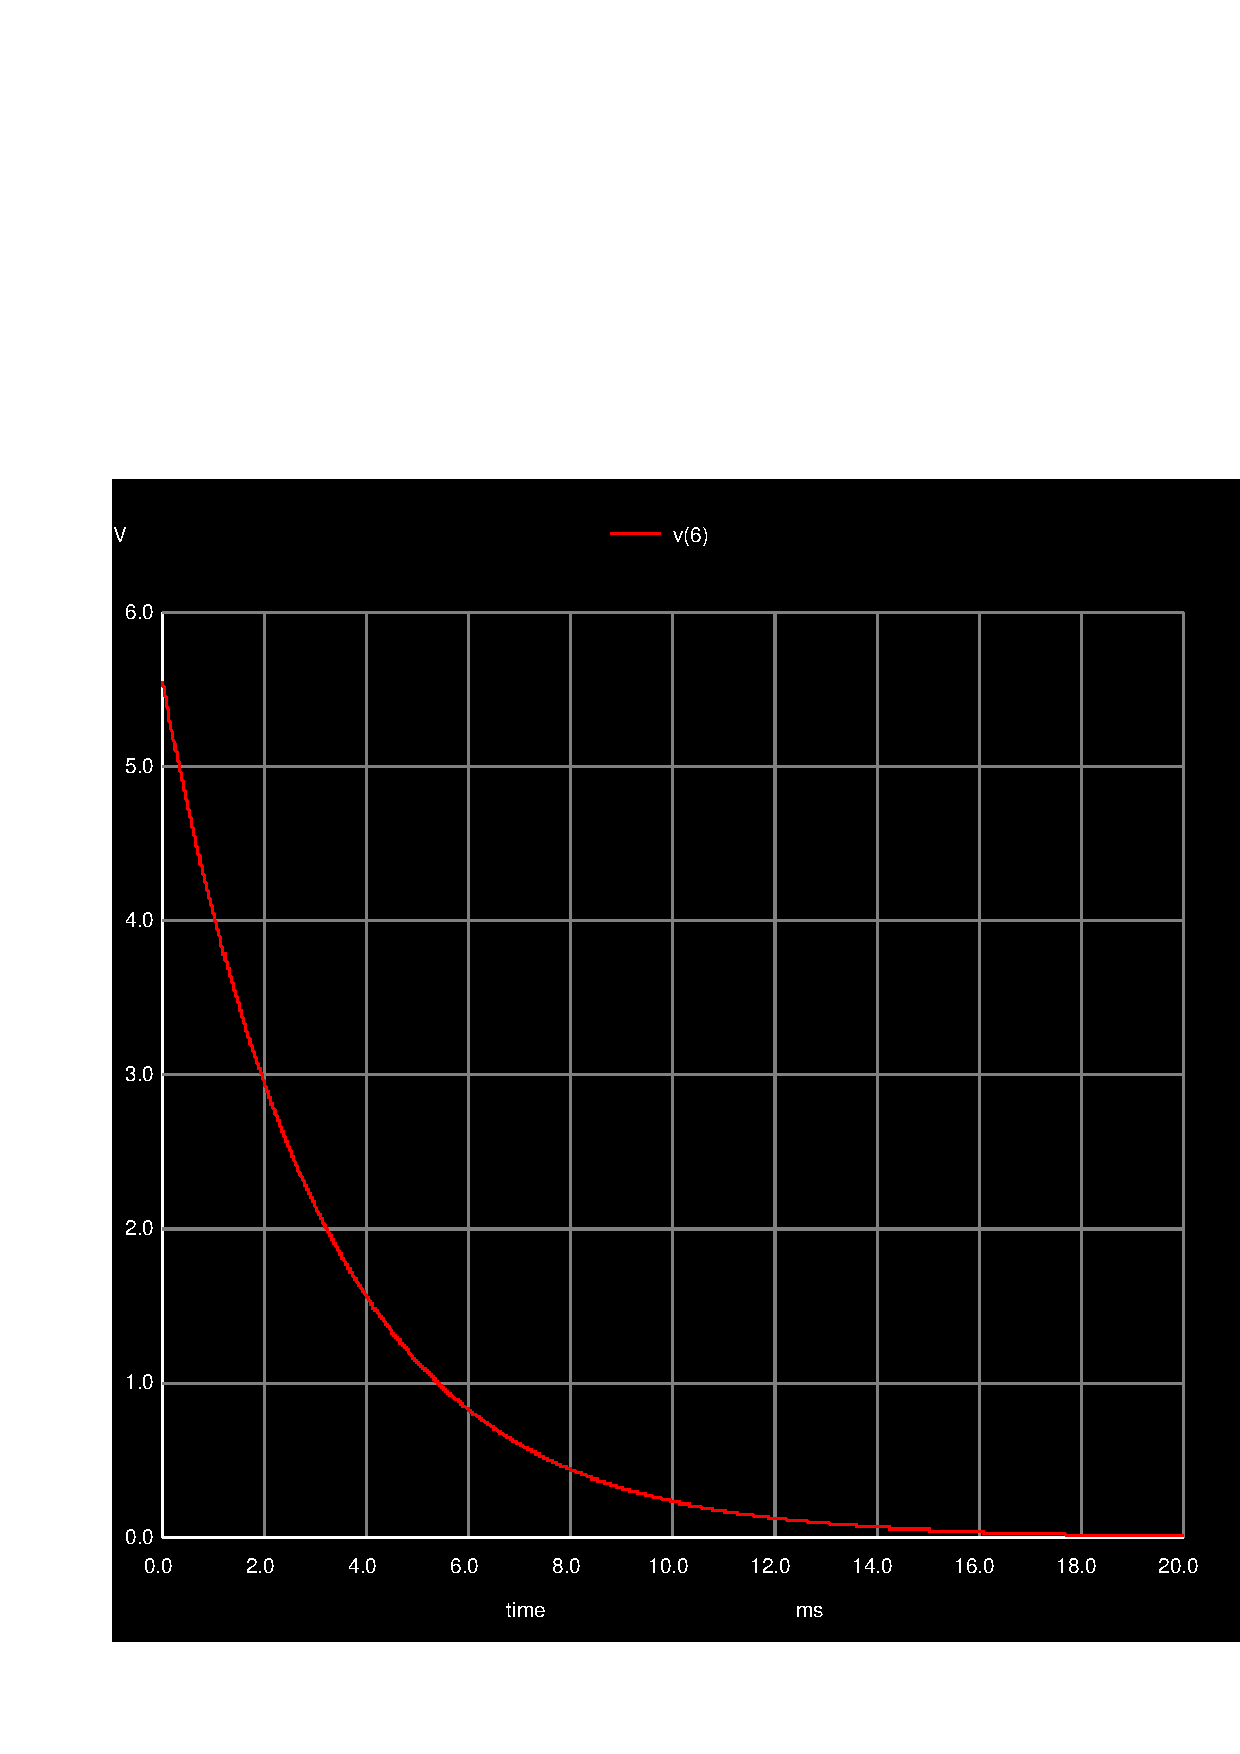
\includegraphics[width=0.6\linewidth]{trans_alinea3.pdf}
  \caption{Transient output voltage of node 6 }
  \label{fig:trans_al3}
  \end{figure}

-----------------------------------------------
-----------------------------------------------
-----------------------------------------------
-----------------------------------------------
-----------------------------------------------
-----------------------------------------------
-----------------------------------------------
-----------------------------------------------

